%---------------------------------------------------------------------------------------
\begin{frame}
\frametitle{Efecto t\'unel cu\'antico}

\begin{figure}[h!]
\centering
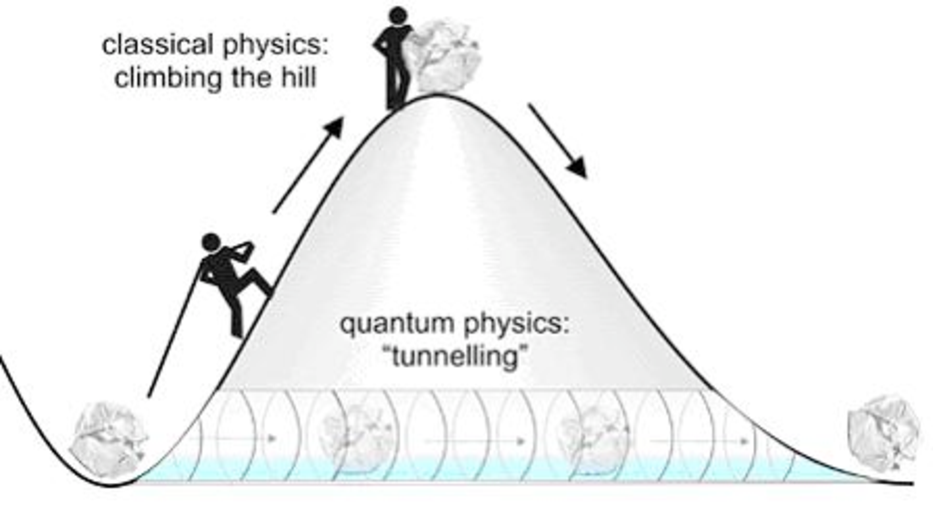
\includegraphics[width=0.7\textwidth]{tunnelling}
\end{figure}

Coeficiente de transmisi\'on: $T \propto e^{-d}$ \hspace{0.5cm} si $\rho d >>1$, $\rho=\sqrt{\frac{2m(V_0-E)}{\hbar^2}}$

\pause
\begin{center}
Pero lo que tenemos nosotros es... \textcolor{red}{una transici\'on discreto $\rightarrow$ cont\'inuo !!}

\vspace{0.3cm}
$\Downarrow$

\vspace{0.3cm}
\textcolor{blue}{La Regla de Oro de Fermi}
\end{center}

\end{frame}
%---------------------------------------------------------------------------------------
%---------------------------------------------------------------------------------------
\begin{frame}
\frametitle{C\'alculo de I(V) con la Regla de Oro de Fermi 1}

1 \textcolor{blue}{La tasa de transici\'on $W$ de un $e^-$ para pasar de una estado ocupado en la l\'amina 1 a un estado vac\'io de la l\'amina 2:}
\begin{equation}\label{probability1}
W_{1\to 2}^{1e} = \frac{2\pi}{\hbar} |T_{21}|^2 f(\epsilon_{\mathbf{p_1}}) [1-f(\epsilon_{\mathbf{p_2}})]
		\delta(\epsilon_{\mathbf{p_1}}-\epsilon_{\mathbf{p_2}})\delta_{s_1s_2},
\end{equation}

\pause
2 \textcolor{blue}{Asumiremos que el hamiltoniano no depende del \emph{esp\'in} y que acopla d\'ebilmente los eletrodos si el potencial aplicado es peque\~no respecto a $\epsilon_F$.}
$$V < 3meV << 10eV \approx \epsilon_F$$
\textcolor{blue}{As\'i que la tasa total de transici\'on del electrodo 1 al 2 ser\'a:}

\begin{equation}\label{probability3}
W_{1\to 2} = \frac{4\pi}{\hbar} |T|^2 \sum_{\mathbf{p_1},\mathbf{p_2}}  
		f(\epsilon_{\mathbf{p_1}}) [1-f(\epsilon_{\mathbf{p_2}})] 
		\delta(\epsilon_{\mathbf{p_1}}-\epsilon_{\mathbf{p_2}}).
\end{equation}

\pause
\vspace{0.5cm}
\begin{center}
\emph{\textcolor{red}{La tasa de transici\'on en la direcci\'on opuesta es an\'aloga}}
\end{center}

\end{frame}
%---------------------------------------------------------------------------------------
%---------------------------------------------------------------------------------------
\begin{frame}
\frametitle{C\'alculo de I(V) con la Regla de Oro de Fermi 2}

\textcolor{blue}{Expresi\'on para la corriente en la direcci\'on $1\to 2$:}
\begin{equation}\label{current1}
I = e\ (W_{1\to 2} - W_{2\to 1}),
\end{equation}

\pause
\begin{equation}\label{current2}
I = \frac{4\pi e}{\hbar} |T|^2 \sum_{\mathbf{p_1},\mathbf{p_2}}  
		[f(\epsilon_{\mathbf{p_1}})-f(\epsilon_{\mathbf{p_2}})] 
		\delta(\epsilon_{\mathbf{p_1}}-\epsilon_{\mathbf{p_2}})
\end{equation}

\pause
\textcolor{blue}{Momentos $\sim$ cuasicont\'inuo $\Rightarrow$ sumatorios $\sim$ integrales}

\textcolor{blue}{Voltaje V $\Rightarrow$ $\mu_2-\mu_1=eV$}

\begin{equation}\label{current3}
I = \frac{4\pi e}{\hbar}  |T|^2 \int_{-\infty}^{\infty} d\epsilon\ N_1(\epsilon-eV)\ N_2(\epsilon) [f(\epsilon-eV)-f(\epsilon)]
\end{equation}


\end{frame}
%---------------------------------------------------------------------------------------
%---------------------------------------------------------------------------------------
\begin{frame}
\frametitle{Densidad de estados para los 3 tipos de uniones}

\begin{columns}
\begin{column}{0.5\textwidth}
	\begin{figure}[!h] \label{fermi_levels}
	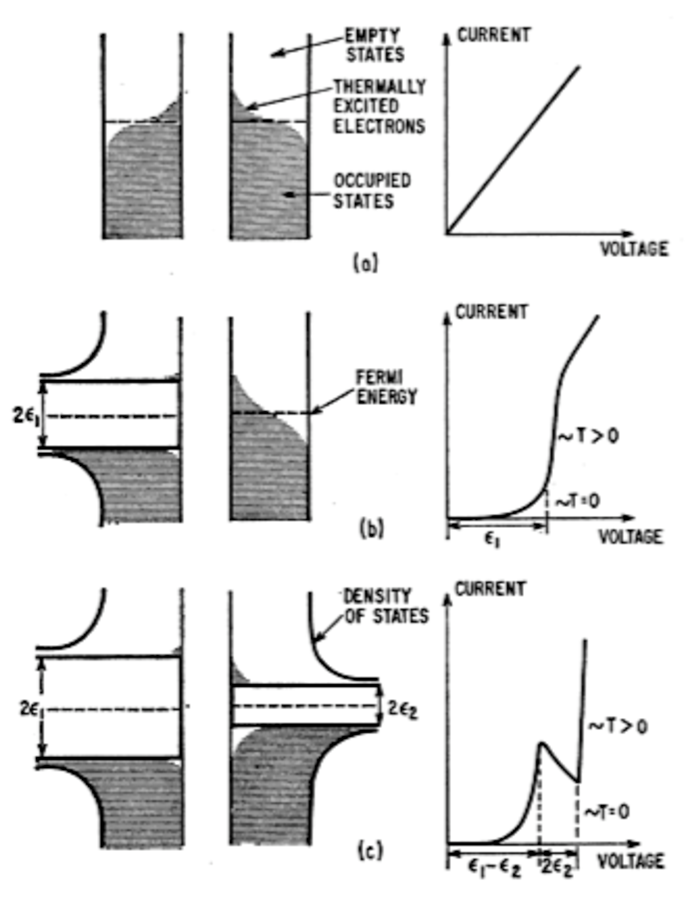
\includegraphics[width=\textwidth]{fermi_levels}
	\end{figure}
\end{column}
\begin{column}{0.5\textwidth}
	\begin{figure}[!h] \label{fermi_levels2}
	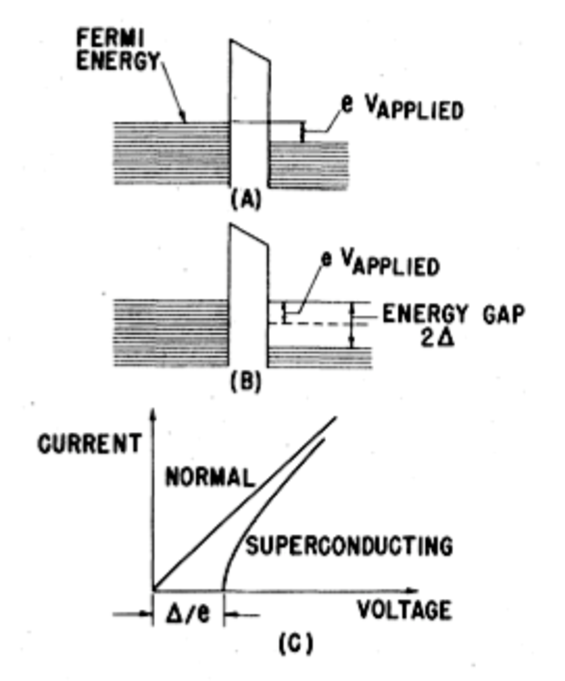
\includegraphics[width=\textwidth]{fermi_levels2}
	\end{figure}
\end{column}
\end{columns}


\end{frame}
%---------------------------------------------------------------------------------------
%---------------------------------------------------------------------------------------
\begin{frame}
\frametitle{Expresiones para I(V) seg\'un BCS en los 3 casos}

\begin{columns}
\begin{column}{0.4\textwidth}
	\begin{figure}[!h] \label{fermi_levels}
	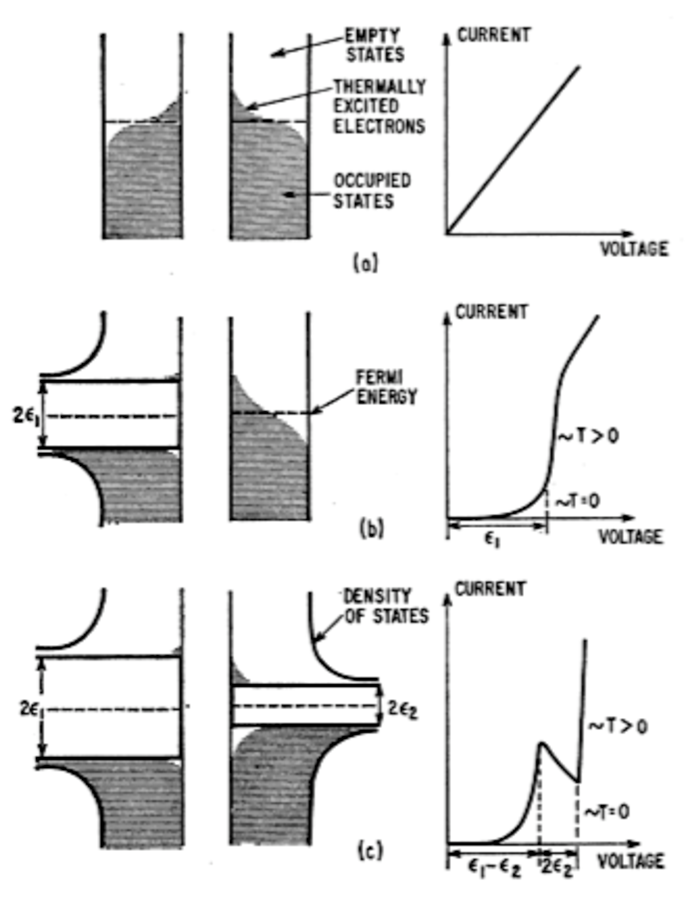
\includegraphics[width=\textwidth]{fermi_levels}
	\end{figure}
\end{column}
\begin{column}{0.6\textwidth}
\begin{flushleft}
	\begin{equation*}\label{inn}
		I^{NN} = \frac{4\pi e}{\hbar} |T|^2 N_1(\mu)N_2(\mu) eV
	\end{equation*}
	\begin{equation*}\label{cnn}
		C^{NN} = \frac{4\pi e}{\hbar} |T|^2 N_1(\mu)N_2(\mu) e
	\end{equation*}
\vspace{0.7cm}
	\begin{equation*}\label{ins}
		I^{NS} = \frac{C^{NN}}{e} \int_{-\infty}^{\infty} dE\ \frac{|E|}{\sqrt{E^2-\Delta^2}} [f(E-eV)-f(E)]
	\end{equation*}
\vspace{0.7cm}	
	\begin{equation*}\label{iss}
		I^{SS} = \frac{C^{NN}}{e} \int_{-\infty}^{\infty} dE\ 
		\frac{E^2\ [f(E-eV)-f(E)]}{\sqrt{(E^2-\Delta_1 ^2)}\sqrt{(E^2-\Delta_2 ^2)}}
	\end{equation*}
\end{flushleft}
\end{column}
\end{columns}

\end{frame}
%---------------------------------------------------------------------------------------
%---------------------------------------------------------------------------------------
\begin{frame}
\frametitle{Curva te\'oricas I(V) 1/2}

\begin{figure}[!h] \label{iv_teorico}
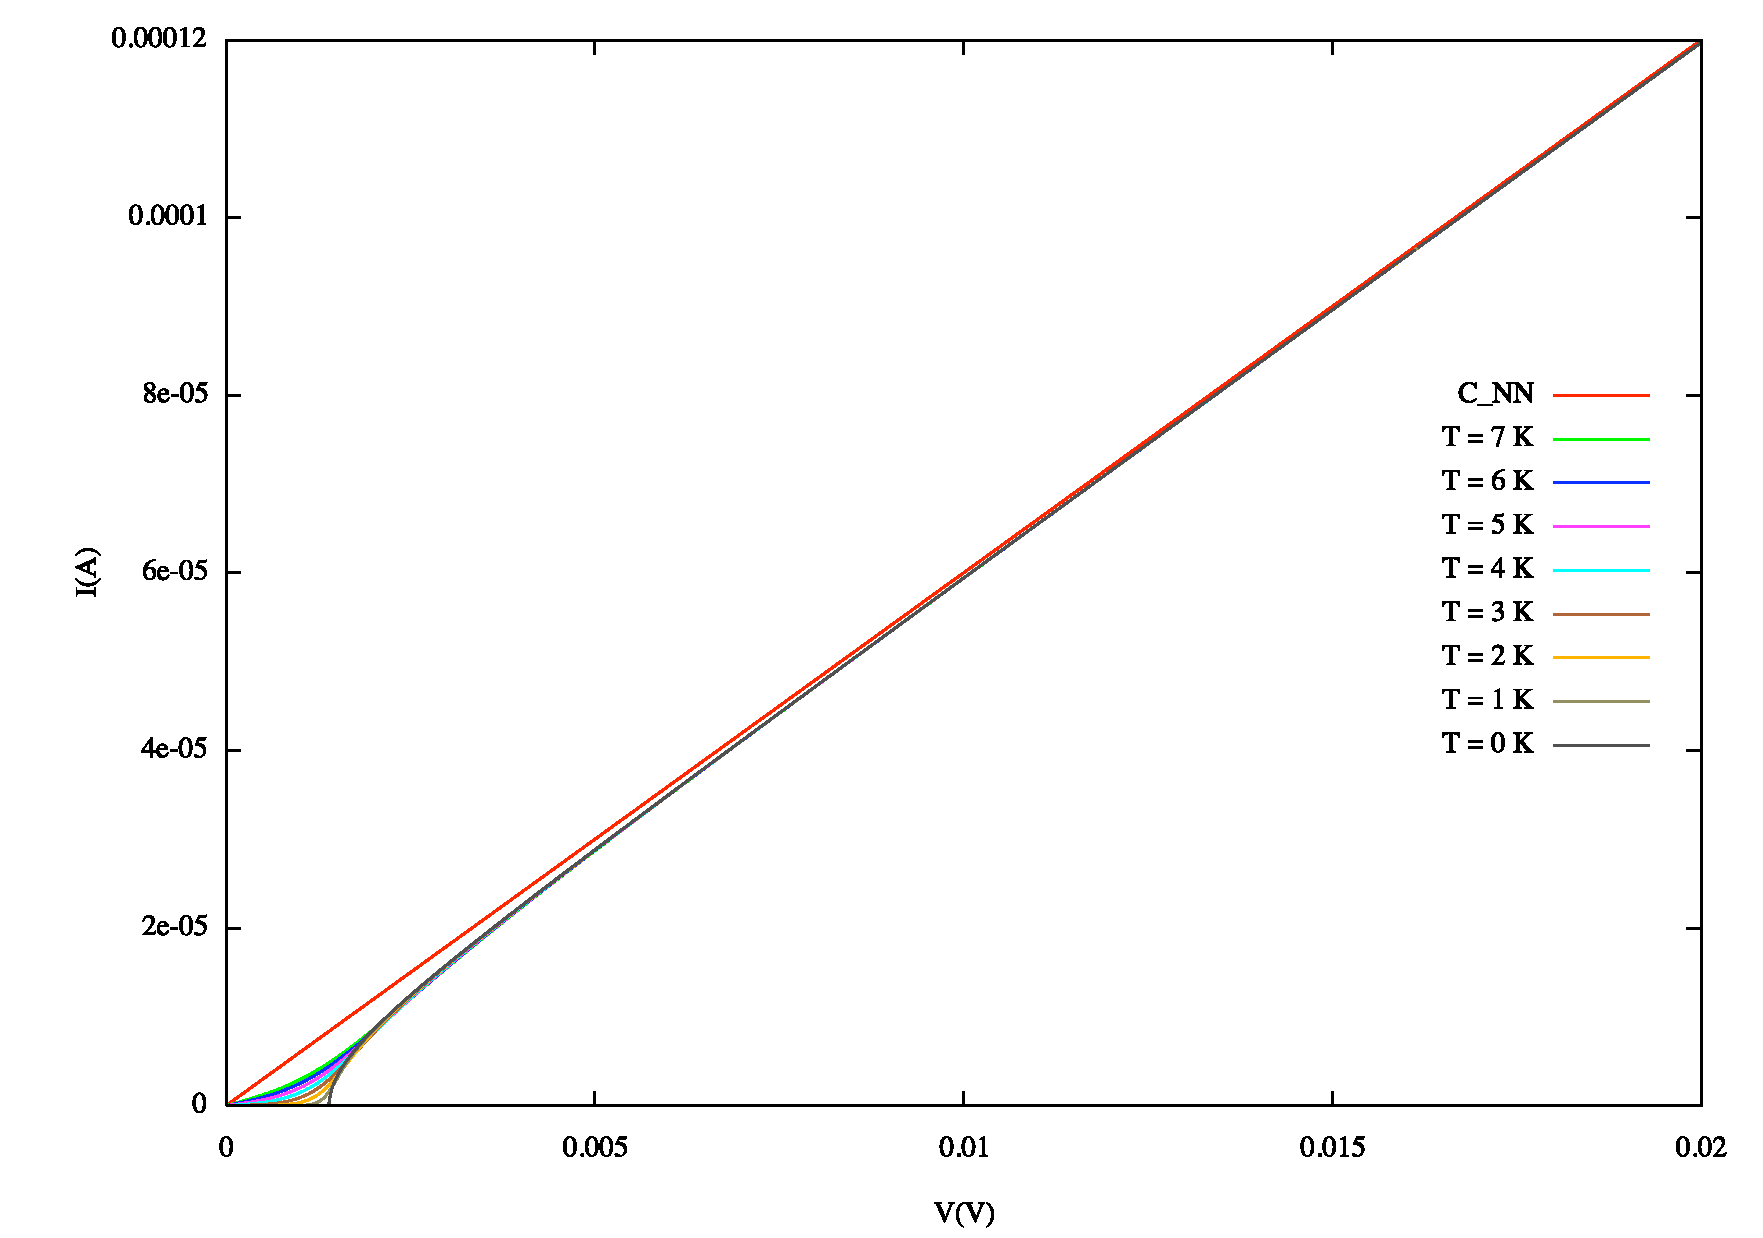
\includegraphics[width=\textwidth]{iv_teorico}
\end{figure}
	
\end{frame}
%---------------------------------------------------------------------------------------
%---------------------------------------------------------------------------------------
\begin{frame}
\frametitle{Curva te\'oricas I(V) 2/2}

\begin{figure}[!h] \label{iv_teorico2}
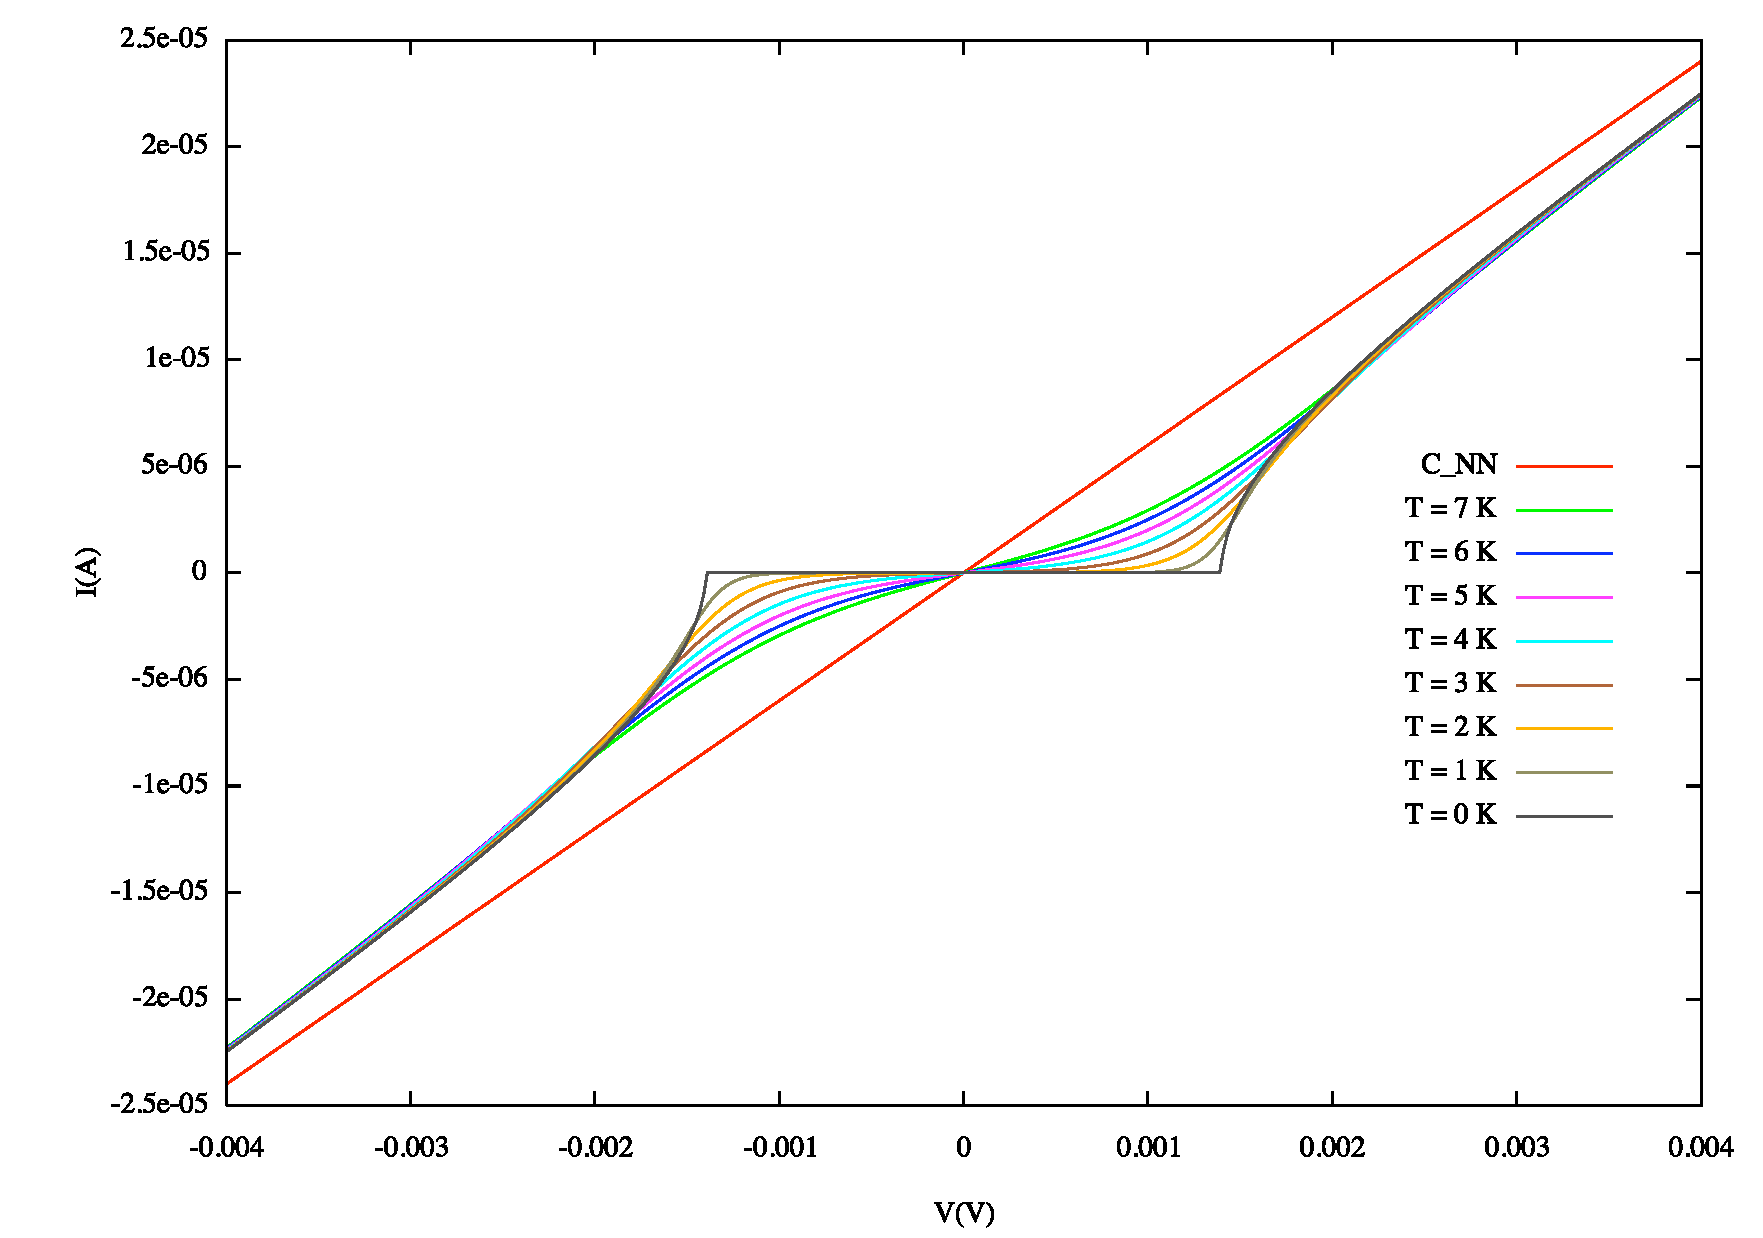
\includegraphics[width=\textwidth]{iv_teorico2}
\end{figure}

\end{frame}
%---------------------------------------------------------------------------------------
%---------------------------------------------------------------------------------------
\begin{frame}
\frametitle{Curva te\'oricas G(V)}

\begin{figure}[!h] \label{gv_teorico}
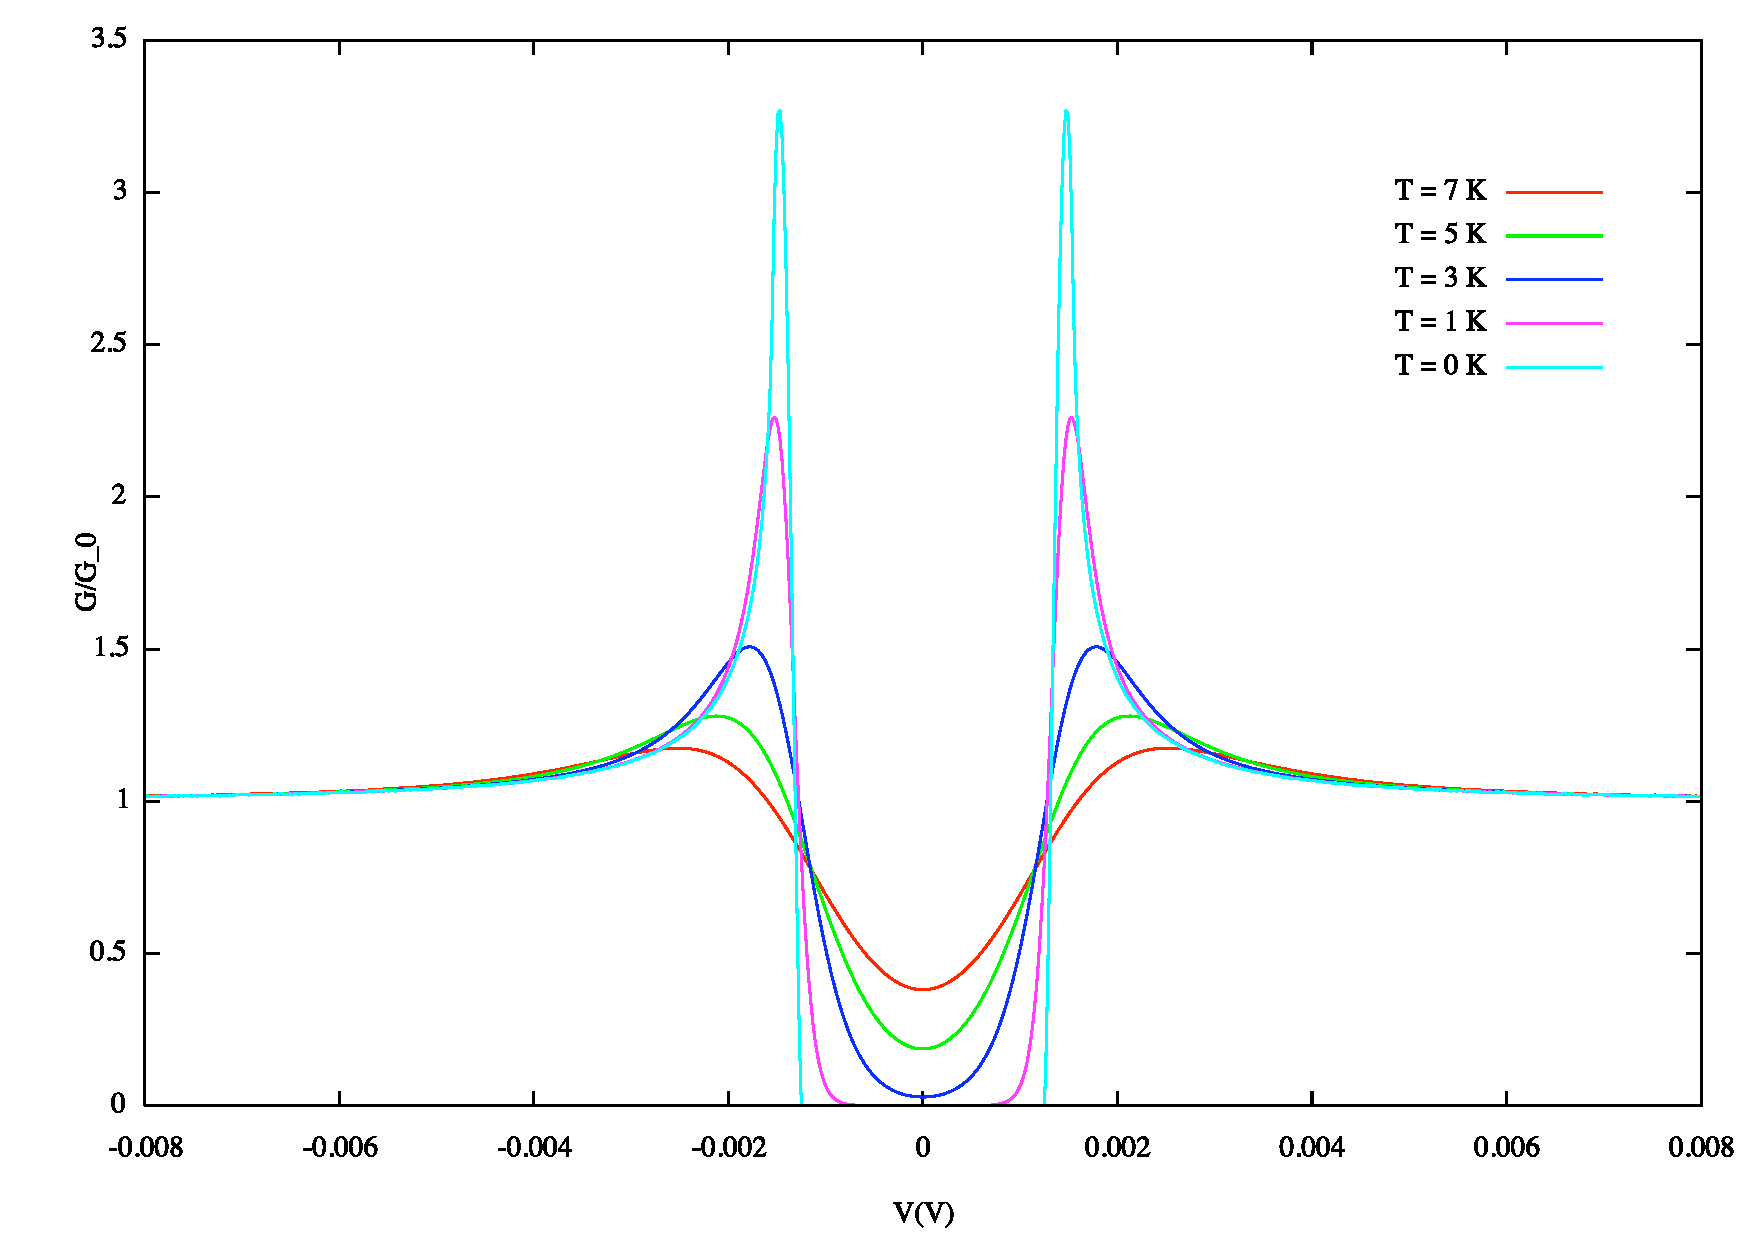
\includegraphics[width=\textwidth]{gv_teorico}
\end{figure}

\end{frame}
%---------------------------------------------------------------------------------------


